\chapter{Anexo I - Pliego de condiciones}
\label{ch:anexoPliegoCondiciones}
%Este anexo se ha añadido siguiendo la recomendación oficial de la \gls{uah} sobre \gls{tfg}s. En él se indicarán las condiciones materiales de las distintas máquinas donde se ha desarrollado el proyecto. Por último, se resumirán tanto las limitaciones de \textit{hardware}, como las especificaciones del \textit{software} instalado en las máquinas virtuales donde se llevó a cabo los distintos casos de uso. 

En este anexo se podrán encontrar las condiciones materiales de las distintas máquinas donde se ha llevado a cabo el desarrollo y evaluación del proyecto. De forma adicional, se han indicado las limitaciones \textit{hardware} así como las especificaciones \textit{software} para poder replicar el proyecto de manera íntegra en otro sistema.


\section{Condiciones materiales y equipos}

%En el siguiente listado se presentan todos los materiales empleados en el proyecto, detallando únicamente las características esenciales de aquellos que fueron cruciales para el desarrollo del \gls{tfm}. De esta manera, se garantiza que todas las especificaciones técnicas utilizadas en las pruebas y validaciones del proyecto queden debidamente registradas.

A continuación, se presentan todas las máquinas empleadas en el desarrollo del proyecto, indicando únicamente aquellas características relevantes para la ejecución del \gls{tfm}. De esta forma, se quiere garantizar que en caso de que se replique las pruebas y validaciones del proyecto se obtengan los mismos resultados, siendo el entorno completamente replicable.

\subsection{Especificaciones Máquina A}
\label{maquina_A}
\begin{itemize}
    \item Procesador: i7-8700K (12) @ 4.700GHz
    \item Memoria: 15674MiB
    \item Gráfica: Intel UHD Graphics 630
    \item Sistema operativo: Ubuntu 20.04.6 LTS x86\_64
\end{itemize}
\begin{figure}[ht!]
    \centering
    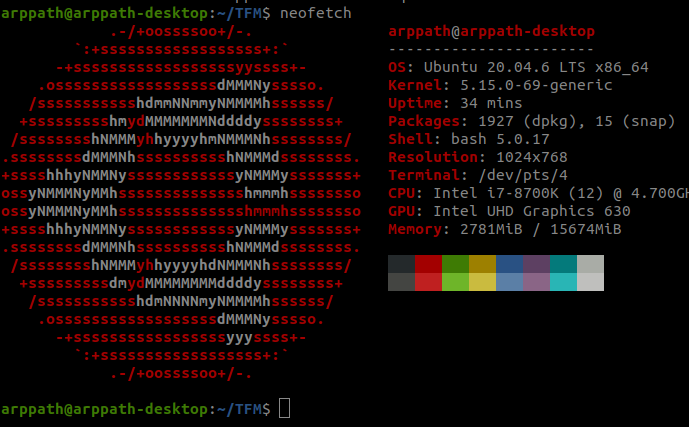
\includegraphics[width=8cm]{archivos/img/anexos/maquinaA.png}
    \caption{Especificaciones de la máquina A}
    \label{fig:maquinaA}
\end{figure}


\subsection{Especificaciones Máquina B}
\label{maquina_B}
\begin{itemize}
    \item Procesador: Intel i5-7500 (4) @ 3.800GHz
    \item Memoria: 31984MiB
    \item Gráfica: Intel HD Graphics 630
    \item Sistema operativo: Ubuntu 22.04.2 LTS x86\_64
\end{itemize}
\begin{figure}[ht!]
    \centering
    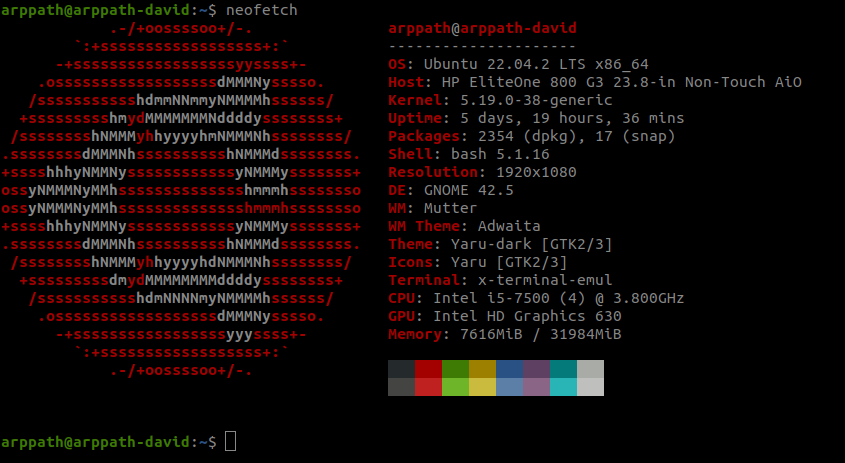
\includegraphics[width=\textwidth]{archivos/img/anexos/maquinaB.png}
    \caption{Especificaciones de la máquina B}
    \label{fig:maquinaB}
\end{figure}

\newpage

\subsection{Especificaciones Máquina C}
\label{maquina_C}
\begin{itemize}
    \item Procesador: Intel(R) Core(TM) 12th Gen i7-1260P (16) CPU @ 4.70Ghz
    \item Memoria: 15674MiB
    \item Gráfica: Intel Alder Lake-P
    \item Sistema operativo: Ubuntu 22.04.2 LTS x86\_64
\end{itemize}
\begin{figure}[ht!]
    \centering
    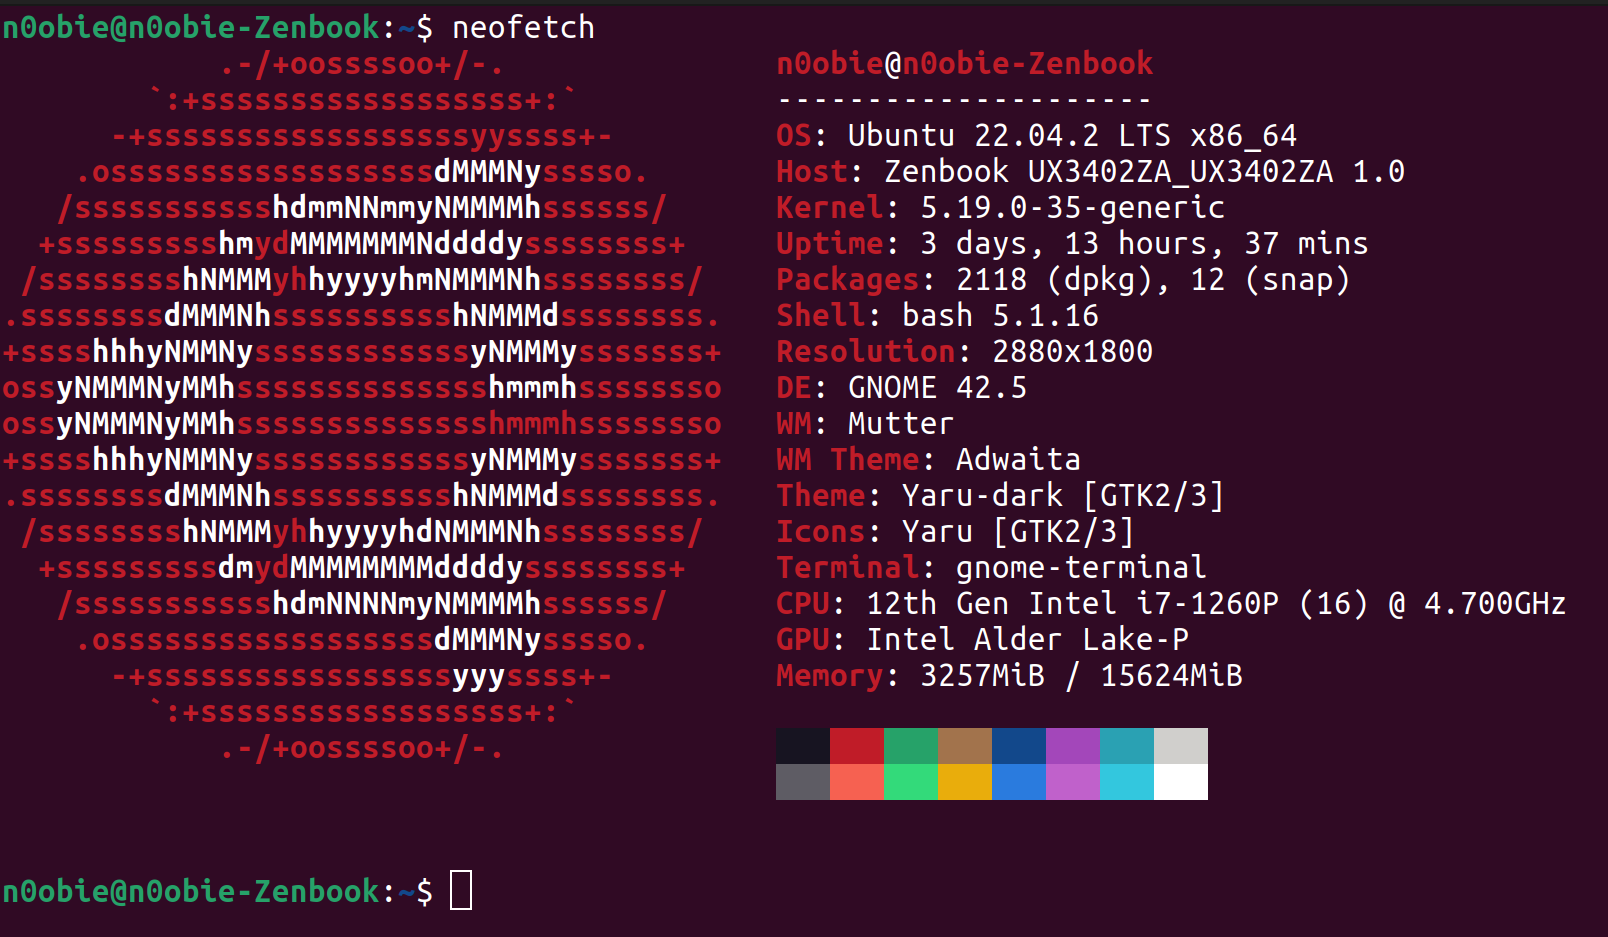
\includegraphics[width=\textwidth]{archivos/img/anexos/maquinaC.png}
    \caption{Especificaciones de la máquina C}
    \label{fig:maquinaC}
\end{figure}
